\documentclass[10 pt,Helvetica, french]{beamer}
% option compress pour réduire la taille des bars
\mode<presentation>
%[compress,hideallsubsections,width=<0.5cm>]
%\usetheme{Darmstadt}
%\usetheme{Malmoe}
%\usetheme{Warsaw}
%\useoutertheme{split}
%\usecolortheme{whale}

%\usepackage[dark]{beamerthemesidebar}
%\usepackage{beamerthemeshadow}
%\usepackage{beamerthemesplit}
%\usepackage{beamerthemebars}
%\usepackage{beamerthemeclassic}
\newcommand{\spac}{\rule[0mm]{0mm}{2mm}}
\usepackage{pgf,pgfarrows,pgfnodes,pgfautomata,pgfheaps,pgfshade}
\usepackage{amsmath,amssymb}
\usepackage[english]{babel}
\usepackage{epic,eepic,bez123}
\usepackage{ bbold }
\usepackage{ upgreek }
\usepackage{amsmath}
%\usepackage[T1]{fontenc}
%\usepackage[ansinew]{inputenc}
%\usepackage[latin1]{inputenc}
%\usepackage{babel,varioref}

%\usetheme{Luebeck}%(encadrements rectangulaires)
%\usetheme{Madrid}%(pas de plan au-dessus)
%\usetheme{Berkeley}%(colonne à gauche)
%\usetheme{Warsaw}%(plan détaillé en haut, utilise la navigation)
%\usetheme{Dresden}%(encadrements rectangulaires)
%\usetheme{Frankfurt}%(pas de paln détaillé en haut)
%\usetheme{Marburg}%(colonne à droite)
%\usetheme{Berlin}%(encadrements rectangulaires)
%\usetheme{Montpellier}

%\usecolortheme{crane}
%\usecolortheme{seahorse}
%\usecolortheme{green}
%\usecolortheme{beetle}
%\usecolortheme{default}
%\usecolortheme{rose}
%\usecolortheme{Berkeley}(inconnu)

%\useoutertheme{smoothtree}
%\useoutertheme{split}
%\usecolortheme{whale}

\setbeamercovered{transparent}
\newtheorem{defi}{Definition}
\newtheorem{theo}{Theorem}
\newtheorem{prop}{Proposition}
\newtheorem{property}{Property}
\newtheorem{coro}{Corollary}
\newtheorem{propannex}{Proposition}
\newtheorem{objective}{Objective}
\newtheorem{res}{Results}


\setbeamertemplate{footline}[text line]{  }
%\setbeamertemplate{footline}[page number]{ }

\newcounter{countAnnexA}
\setcounter{countAnnexA}{0}
\renewcommand{\propannex}{\addtocounter{countAnnexA}{1}
\noindent \large \textbf{Proposition \thesection.\thecountAnnexA}
\normalsize}

\newcommand{\beginbackup}{
   \newcounter{framenumbervorappendix}
   \setcounter{framenumbervorappendix}{\value{framenumber}}
}
\newcommand{\backupend}{
   \addtocounter{framenumbervorappendix}{-\value{framenumber}}
   \addtocounter{framenumber}{\value{framenumbervorappendix}}
}

%\colorlet{orange}{red!70!yellow}% mes petites couleurs que j'aime bien
%\colorlet{mauve}{blue!70!red} \colorlet{brouge}{red!70!blue}
\addtobeamertemplate{footline}{\insertframenumber/\inserttotalframenumber}


\date[September 2016]{ETSG, Helsinki, September 2016}
\title[Trade Costs Black Box]{Beyond the Iceberg Hypothesis: \\Opening the Black Box of Transport Costs}
\author[Daudin et al.]{Guillaume Daudin\\
{\footnotesize Universit\'{e} Paris-Dauphine, PSL \& OFCE }\\ \smallskip
J\'{e}rome H\'{e}ricourt \\
{\footnotesize Universit\'{e} de Lille I \& CEPII }\\  \smallskip
Lise Patureau \\
{\footnotesize  Universit\'{e} Paris-Dauphine, PSL}}


\setcounter{framenumber}{-1}
\begin{document}
\begin{frame}[plain]
\titlepage
\end{frame}


\begin{frame}
\frametitle{Motivation}
\begin{itemize}
\item Trade costs: A central role in international economic analysis \vspace{0.1cm}
\begin{itemize}
\item[-] Declining over the second half of the 20$^{th}$ century (Jacks et al., 2008, Novy, 2013) \vspace{0.1cm}
\item[-] But still significant: Average international trade costs = a 74\% markup over production costs (Anderson \& Van Wincoop, 2004)
\end{itemize}
\item What exactly are ``trade costs''?  \vspace{0.1cm}
\begin{itemize}
\item[-] Transaction costs, policy costs, time costs, and transport costs \textit{per se}
\end{itemize}
\item Transport costs: A sizeable share of international trade costs \vspace{0.1cm}
\begin{itemize}
\item[-] Account for 21\% of international trade costs $\Leftrightarrow$ A 15\% markup (Anderson \& Van Wincoop, 2004) \vspace{0.1cm}
%\item[-] Elasticity of trade wrt freight costs = -3 (Behar \& Venables, 2011) \vspace{0.1cm}
\end{itemize}
\item[$\Rightarrow$] If many trade policy barriers have been removed, the transport cost component of trade costs does not seem to be declining\vspace{0.1cm}
\end{itemize}
\textbf{The paper: On international transport costs}

\end{frame}

\begin{frame}
\frametitle{Motivation (cont')}
\begin{itemize}
\item Standard modeling of trade costs: As an ad-valorem tax-equivalent \vspace{0.1cm}
\begin{itemize}
\item[-] As a constant percentage of the producer price per unit traded \vspace{0.1cm}
\item[$\Leftrightarrow$] The ``iceberg cost'' hypothesis (Samuelson, 1954) \vspace{0.1cm}
\end{itemize}
\item Yet... A debated question \vspace{0.1cm}
\item Would not trade costs rather exhibit an additive structure ?  \vspace{0.1cm}
\item The structure (additive vs iceberg) of transport costs, not anecdotal \vspace{0.1cm}
\begin{itemize}
\footnotesize{
\item[-] Additive trade costs \& the pattern of trade flows (Alchian \& Allen, 1964) \vspace{0.1cm}
\item[-] Strong normative implications (Sorensen, 2014)\vspace{0.1cm}
\item[-] The additive structure of trade costs is supported by recent empirical evidence (Hummels \& Skiba, 2004)  \vspace{0.1cm}}
\end{itemize}
\item[$\Rightarrow$] Trade costs are likely to display an additive component, but precisely... by how much? \vspace{0.1cm}
\end{itemize}
\textbf{One objective of the paper: Provide an answer to this question}
\end{frame}

\begin{frame}
\frametitle{Our paper in 3 questions (and 3 answers)}
An empirical decomposition of the structure of transport costs \vspace{0.1cm}
\begin{itemize}
\item[(1)] What is the size of the iceberg and the additive trade costs? \vspace{0.1cm}
\item[$\Rightarrow$] Provide a quantitative measure of both, using US imports data \vspace{0.1cm}
\begin{itemize}
\footnotesize{
\item[-] Iceberg cost: 2.5\% and 3.2\% of the export price in air and ocean transport (mean value over 1974-2013, US imports) \vspace{0.1cm}
\item[-] Additive cost: 1.8\% and 2.9\% of the export price  \vspace{0.1cm}
}
\end{itemize}
\item[(2)] What do we lose by skipping the additive part of transport costs? \vspace{0.1cm}
\item[$\Rightarrow$] We lose much: With the additive term included, \vspace{0.1cm}
\begin{itemize}
\item[-] The estimated iceberg component is reduced by a factor of 2 \vspace{0.1cm}
\item[-] A significantly better ``goodness-of-fit'' \vspace{0.1cm}
\end{itemize}
\item[(3)] How have international transport costs evolved over time? \vspace{0.1cm}
\begin{itemize}
\item[-] Transport costs \textit{per se} have fallen since 1985, by $\simeq$ 40\% \vspace{0.1cm}
\item[-] When additive costs are included, not much difference between air and sea transport, $\neq$ Hummels (2007) and Behar \& Venables (2010) \vspace{0.1cm}
%\item[-] Marked difference in the evolution of additive and multiplicative costs in Air
\end{itemize}
\end{itemize}
\end{frame}

\begin{frame}
\frametitle{Outline of the talk}
\begin{itemize}
\item Data Sources  \vspace{0.1cm}
\item Empirical Methodology \vspace{0.1cm}
\item Results \vspace{0.1cm}
\item Conclusion
\end{itemize}
\end{frame}

\begin{frame} [label=slide_data]
\frametitle{Data sources}
\begin{itemize}
\item Our measure of international transport costs: The difference between the export ($\simeq$ fas) price and the import (cif) price \vspace{0.1cm}
\item Database: US Imports of Merchandise database \hyperlink{app_data}{\beamergotobutton{More}}\vspace{0.1cm}
\begin{itemize}
\item[-] The export (fas) price, $\widetilde{p}$: the price for one kg of merchandise at the country export point \vspace{0.1cm}
\item[-] The import (cif) price, $p$: the price for one kg of merchandise at the entry in the US \vspace{0.1cm}
\item[-] Yearly basis, from 1974 to 2013, HS 10 digit classification level, by transport mode (air or vessel) \vspace{0.1cm}
\item[-] A dataset also used by Hummels (2007) (until 2004) \vspace{0.1cm}
\end{itemize}
\item[$\Rightarrow$] Our dependent variable: The ratio $p/\widetilde{p}$ \vspace{0.1cm}
\begin{itemize}
\item[-] At the 3-digit classification level  \vspace{0.1cm}
\item[-] At the 4-digit level on some selected years as robustness check \vspace{0.1cm}
\item[-] Approximatively 200 products (3 digits), from around 200 countries  \vspace{0.1cm}
\begin{itemize}
\item[$\ast$] Around 600-700 products at the 4-digit level
\end{itemize}
\end{itemize}
\end{itemize}
\end{frame}


\begin{frame}
\frametitle{Empirical specification: The estimated equation}
\begin{itemize}
\item Relate the import price $p$ to the export price $\widetilde{p}$ given both additive (per-kg) costs $t$ and ad-valorem costs $\tau$:
$$p = \tau \widetilde{p} + t, \qquad \text{with}\quad \tau \geq 1,\quad t \geq 0$$
\item For product $k$, from country $i$  \vspace{0.1cm}
\item Rewrite to get:
$$\frac{p_{ik}}{\widetilde{p}_{ik}} -1 = \tau_{ik} -1 +\frac{t_{ik}}{ \widetilde{p}_{ik}}$$
\item[$\Rightarrow$] Estimate this equation for each year over 1974-2013 \vspace{0.1cm}
\begin{itemize}
\item[-] The equation being also year- and mode (air or vessel)- specific
\end{itemize}

\end{itemize}
\end{frame}

\begin{frame}  [label=slide_method]
\frametitle{Empirical specification: The estimation strategy }
\begin{itemize}
\item With some assumptions on the specification of transport costs \& the error term, and taking logs  \hyperlink{app_method_1}{\beamergotobutton{More}}\vspace{0.1cm}
\item[$\Rightarrow$] Estimate the following equation \vspace{0.1cm}
\footnotesize
\begin{equation}
\ln\left(\frac{p_{ik}}{\widetilde{p}_{ik}}-1 \right)= \ln \left(\tau_{i} \times \tau_{k}+\frac{t_{i} + t_{k}}{\widetilde{p}_{ik}}-1 \right) + \epsilon_{ik} \label{eq:model_with_add}
\end{equation}
\begin{itemize}
\item[-] Estimates performed using non-linear least squares \hyperlink{app_method_2}{\beamergotobutton{More}} \vspace{0.1cm}
\end{itemize}
\normalsize
\item How to characterize the importance of additive costs relatively to iceberg? \vspace{0.1cm}
\item[$\Rightarrow$] Estimate Equation (\ref{eq:model_with_add}) constraining $t=0$:
\footnotesize
\begin{equation}
\ln\left(\frac{p_{ik}}{\widetilde{p}_{ik}}-1 \right)= \ln \left(\tau_{i} \times \tau_{k}-1 \right) + \epsilon^{ice}_{ik} \label{eq:model_nlI}
\end{equation}
\normalsize
\item  Taking the weighted average over the product-country dimension, we finally get (by year and transport mode): \hyperlink{app_method_2}{\beamergotobutton{More}}\vspace{0.1cm}
\begin{itemize}
\item[-] When additive costs are included: $\widehat{\tau}^{adv}$, $\widehat{t}^{add}$  \vspace{0.1cm}
\item[-] With only ad-valorem costs: $\widehat{\tau}^{ice}$
\end{itemize}
\end{itemize}
\end{frame}

\begin{frame}[label=slide_results_summary]
\frametitle{Result 1: Estimating transport costs over time}
For both the ad-valorem and the additive components \vspace{0.1cm}
\begin{itemize}
\item[-] \footnotesize{Average values over 1974-2013, in percent of the export price \hyperlink{app_results_summary}{\beamergotobutton{More}}  } \vspace{0.1cm}
\end{itemize}
\begin{table}[htbp]
  \centering
  \scriptsize{
  %\caption{Transport costs estimates: Summary \label{tab:summary_results}}
  \begin{center}
    \begin{tabular}{l|cc|cc}
      \hline \hline
    %\multicolumn{5}{c}{Mean value over 1974-2013}   \\
    \# digit & \multicolumn{2}{c}{3 digits} & \multicolumn{2}{c}{4 digits} \\ \hline
    Mode  & Vessel & Air & Vessel & Air \\ \hline
    \multicolumn{5}{l}{With only Ad-Valorem Trade Costs ($\widehat{\tau}^{ice}$)}  \\ \hline
    Mean  & \bf{5.8} & \bf{5.1} & 6.0 & 4.9 \\
    Median & 5.1 & 4.2 & 5.2 & 3.7 \\ \hline
    %Std   & 0.032 & 0.042 & 0.036 & 0.045 \\
    %Min. value & 1.003 & 1.001 & 1.003 & 1.000 \\
    %Max. value & 1.304 & 1.685 & 1.408 & 2.051 \\ \hline
    \multicolumn{5}{l}{With Additive \& Ad-Valorem Trade Costs } \\ \hline
   \multicolumn{5}{l}{\textit{Ad-valorem term} ($\widehat{\tau}^{adv}$)}\\ \hline
    Mean  & \bf{3.2} & \bf{2.5} & 3.3 & 2.4 \\
    Median & 2.8 & 1.8 & 2.8 & 1.6 \\ \hline
    %Std   & 0.023 & 0.023 & 0.025 & 0.026 \\
    %Min. value & 1.001 & 1.000 & 1.000 & 1.000 \\
    %Max. value & 1.227 & 1.474 & 1.264 & 1.537 \\ \hline
    \multicolumn{5}{l}{\textit{Additive term }($\widehat{t}^{add}/\widetilde{p}$)} \\ \hline
    Mean  & \bf{2.9} & \bf{1.8} & 2.8 & 1.9 \\
    Median & 1.9 & 0.7 & 1.7 & 0.8 \\ \hline
    %Std   & 0.041 & 0.034 & 0.039 & 0.034 \\
    %Min. value & 0.000 & 0.000 & 0.000 & 0.000 \\
    %Max. value & 2.941 & 13.303 & 3.197 & 11.440 \\ \hline
        \# obs. & 29279 & 28207 & 29317 & 27680 \\ \hline \hline
   % \# origin country & 188 & 191 & 188 & 189 \\
   % \# products & 230 & 211 & 666 & 567 \\
  \end{tabular}
%\parbox[l]{8cm}{\tiny{Notes: Statistics are obtained weighting each observation by its value.}}
%. The additive term is expressed in fraction of fab price. ($^\ast$): Four 4-digit estimation: 0n selected years. ($^{\ast \ast}$): 1989 omitted in 3 digit estimation for air.}}
\end{center}}
  \end{table}%
\begin{itemize}
\item Transport costs are sizeable \vspace{0.1cm}
\begin{itemize}
\item[-] Add $\simeq$ a 5\% margin over the export price \vspace{0.1cm}
\end{itemize}
\item Opening the black box of transport costs \vspace{0.1cm}
\begin{itemize}
\item[-] Iceberg cost: 2.5\% and 3.2\% of the export price in Air \& Vessel resp. 
\item[-] Additive cost: 1.8\% and 2.9\% of the export price 
\end{itemize}
\end{itemize}
\end{frame}

\begin{frame}[label=slide_result2]
\frametitle{Result 2: Additive transport costs do matter}
\begin{itemize}
\item International transport costs: A sizeable additive component \vspace{0.1cm}
\begin{itemize}
\item[-] Omitting the additive term substantially biases the iceberg component upwards (Table 1) \vspace{0.1cm}
\begin{itemize}
\item[$\star$] The ad-valorem cost is reduced by a factor of 2 when additive transport costs are included in the estimation  \vspace{0.1cm}
\item[$\star$] From 5.8\% to 3.2\% in ocean shipping (mean value over the period) \vspace{0.1cm}
\item[$\star$] From 5.1\% to 2.5\% in Air transport \vspace{0.1cm}
\end{itemize}
\item[-] A sizeable share of the additive component in total transport costs \vspace{0.1cm}
\begin{itemize}
\item[$\star$] 48.2\% in average for ocean, 42.3\% for air  \vspace{0.1cm}
\item[$\star$] A result that holds throughout the period \hyperlink{slide_fig1}{\beamergotobutton{See Figure 1 later}} \vspace{0.1cm}
\end{itemize}
\end{itemize}
\item A result confirmed by goodness of fit comparisons \vspace{0.1cm}
\begin{itemize}
\item[-] 4 measures of goodness of fit for Models (\ref{eq:model_with_add}) (with additive TC) and (\ref{eq:model_nlI}) (without additive TC) \vspace{0.1cm}
\item[$\Rightarrow$] A systematically better goodness of fit when including the additive component \hyperlink{app_goodnessfit}{\beamergotobutton{More results}} \vspace{0.1cm}
\begin{itemize}
\item[$\star$] Taking into account the additional degrees of freedom
\end{itemize}
\end{itemize}
\end{itemize}
\end{frame}


\begin{frame}[label=slide_fig1]
\frametitle{Result 3: Characterizing the trends of transport costs }
\begin{itemize}
\item Study the shares of both ad-valorem and additive components in total transport costs  \hyperlink{slide_result2}{\beamergotobutton{Go back to Result 2}} \hyperlink{slide_comment_compositioneffects}{\beamergotobutton{Go back to Result 3}}
\begin{figure}[htbp]
%\caption{Decomposing Transport costs (Yearly mean value, 3 digits)}
%\label{fig:decomp_TC_3d}
\begin{center}
\begin{tabular}{cc}
{\scriptsize (a) Air } & {\scriptsize  (b) Vessel}\\
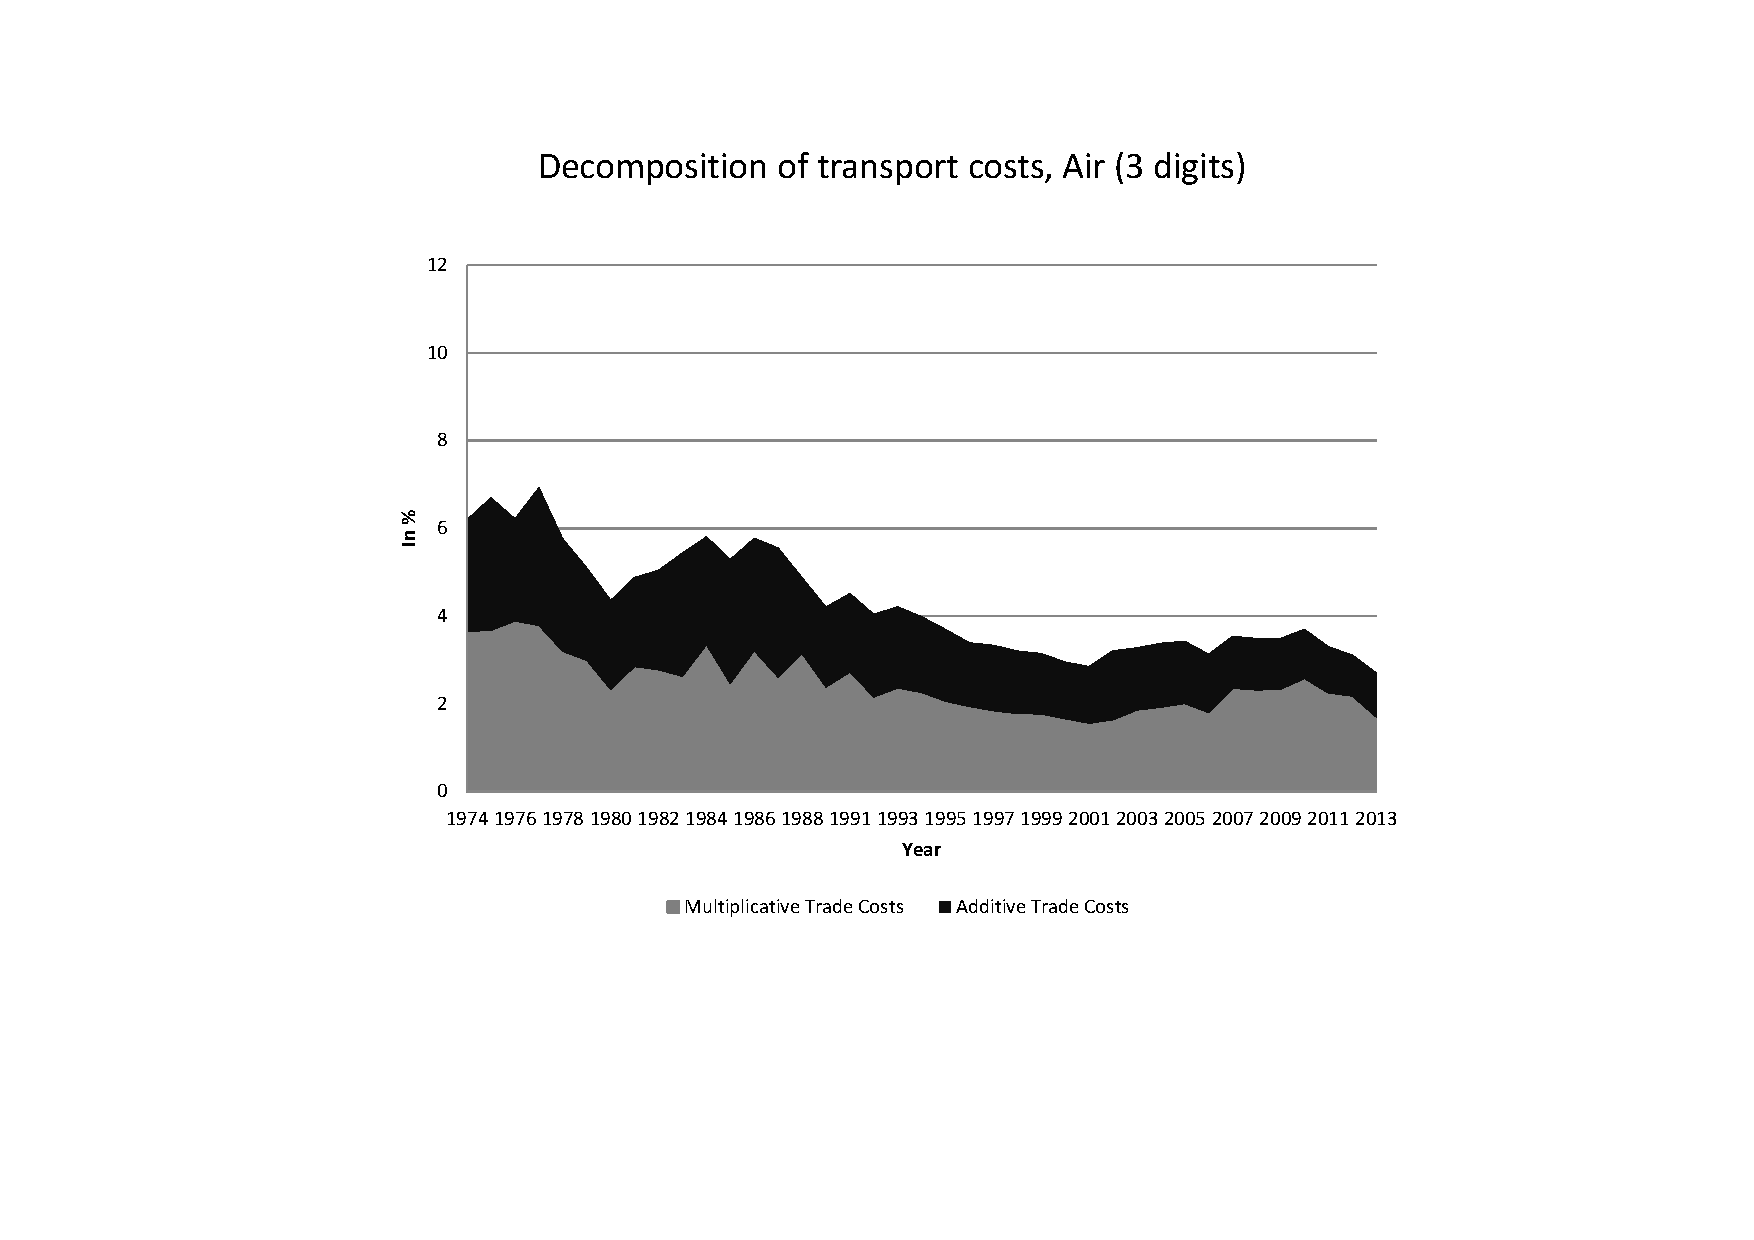
\includegraphics[width=5cm, height=4cm]{Fig2a_decompTC_air_3d.pdf}
& 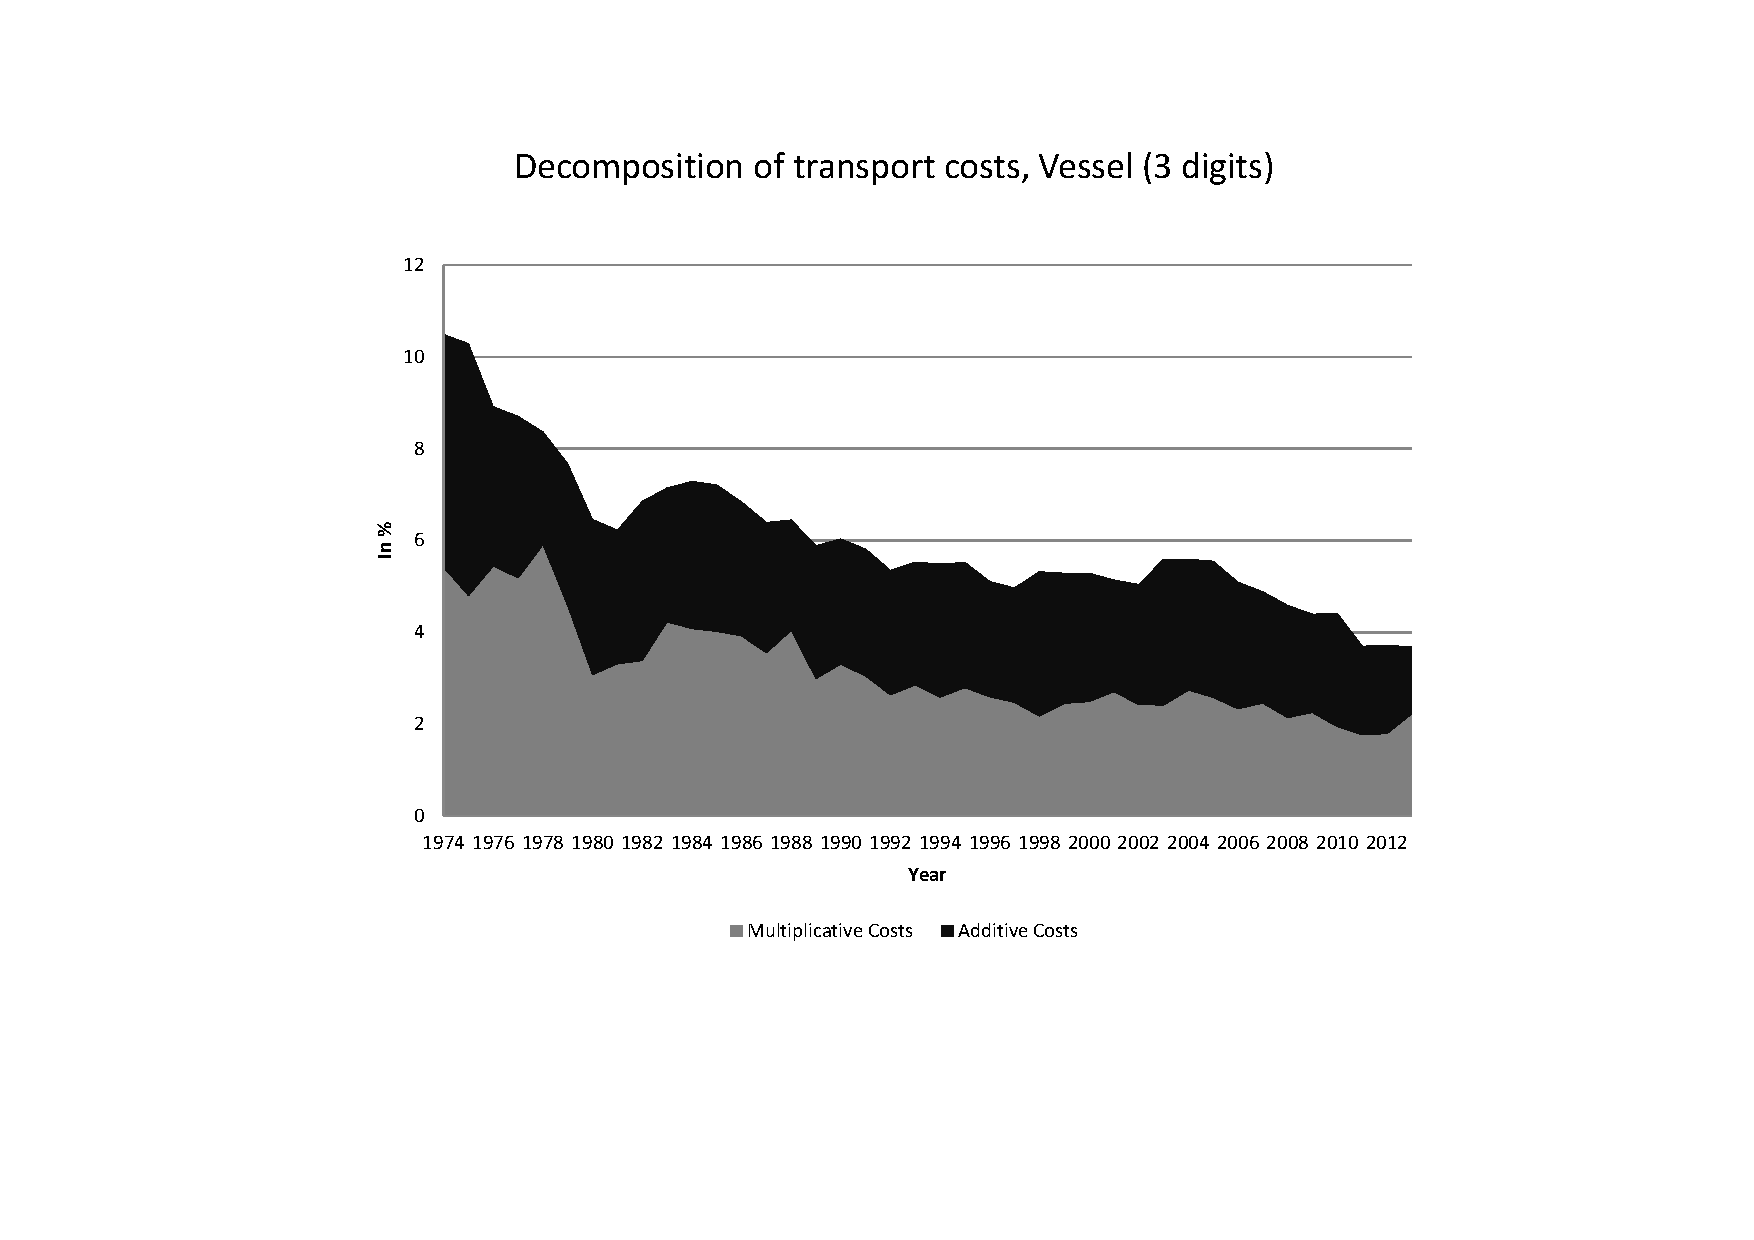
\includegraphics[width=5cm,height=4cm]{Fig2b_decompTC_vessel_3d.pdf} \\
\end{tabular}\end{center}
\end{figure}
\begin{itemize}
\item[-] Lower overall transport costs in Air than in Vessel \vspace{0.1cm}
\item[-] Downward trend for both modes since 1974 \hyperlink{app_fig1}{\beamergotobutton{Robustness of this result}}\vspace{0.1cm}
%\item[-] Slighlty ore pronounced in ocean shipping \vspace{0.1cm}
\begin{itemize}
\item[$\star$] A 50\% decrease in Air, a 60\% decrease in Vessel \vspace{0.1cm}
\end{itemize}
\end{itemize}
\end{itemize}
\end{frame}



\begin{frame}[label=slide_compositioneffects]
\frametitle{Time trends in transport costs \& composition effects }
\begin{itemize}
\item Does it mean a decrease in transport costs \textit{per se}? Not necessarily \vspace{0.2cm}
\item The change in overall transport costs over time: \vspace{0.1cm}
\begin{itemize}
\item[-] Depend on the evolution of per product- per partner costs, \vspace{0.1cm}
\item[-] But also on the composition of trade flows \vspace{0.2cm}
\begin{itemize}
\item[$\star$] Over time, import more goods that are cheaper to transport, and/or from countries with which it is cheaper to trade \vspace{0.1cm}
\end{itemize}
\end{itemize}
\item[$\Rightarrow$] Necessary to eliminate the composition effects of trade flows, to isolate the evolution of transport costs \textit{per se}   \vspace{0.1cm}
\item[$\Rightarrow$] What we do, in accordance with Hummels (2007) \hyperlink{app_compositioneffects}{\beamergotobutton{More on the method}}
\end{itemize}
\end{frame}

\begin{frame}
\begin{itemize}
\item Total transport costs (composition effects excluded) over time
\end{itemize}
\begin{figure}[htbp]
%\caption{Decomposing Transport costs (Yearly mean value, 3 digits)}
%\label{fig:decomp_TC_3d}
\begin{center}
\begin{tabular}{cc}
{\scriptsize (a) Iceberg alone } & {\scriptsize  (b) With additive }\\
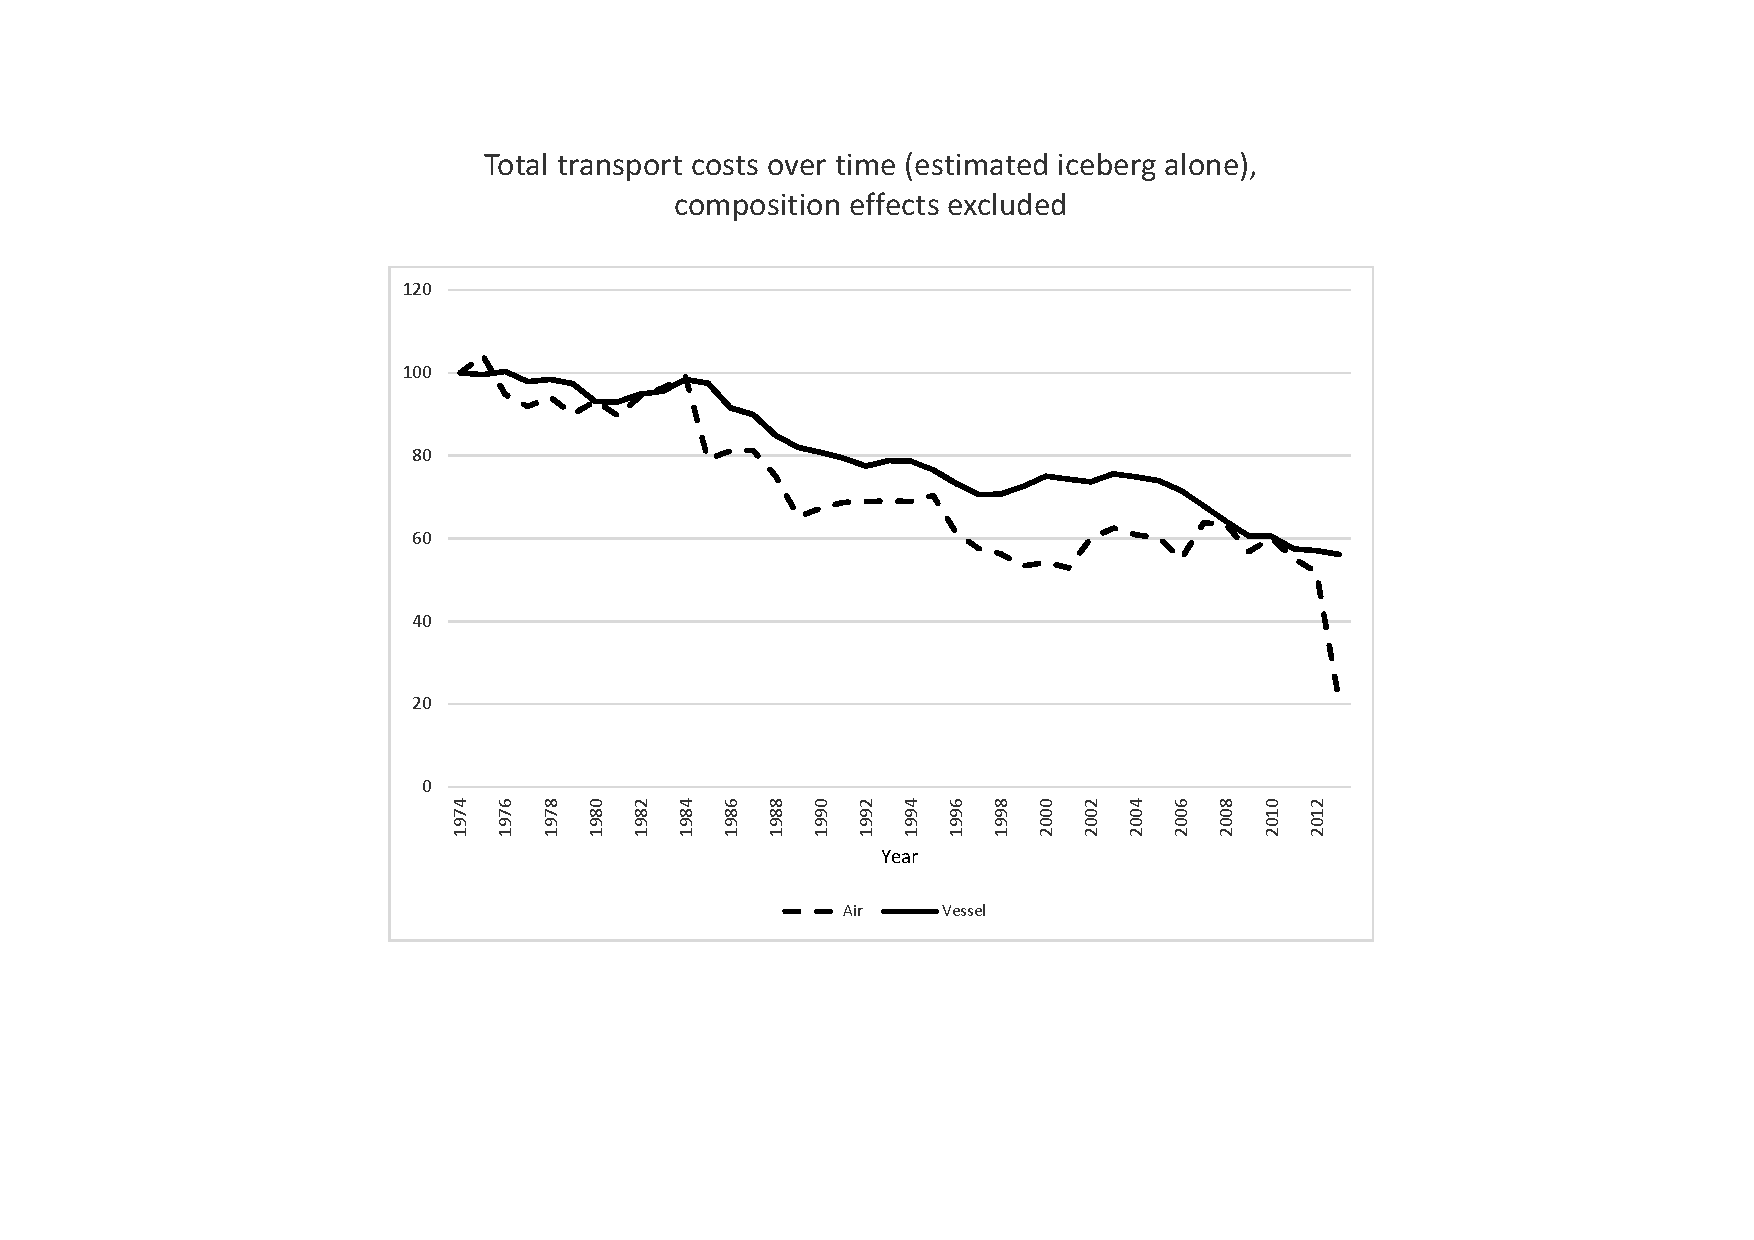
\includegraphics[width=5cm, height=5cm]{Fig3a_TC_overtime_comp_effects_excl.pdf}
& 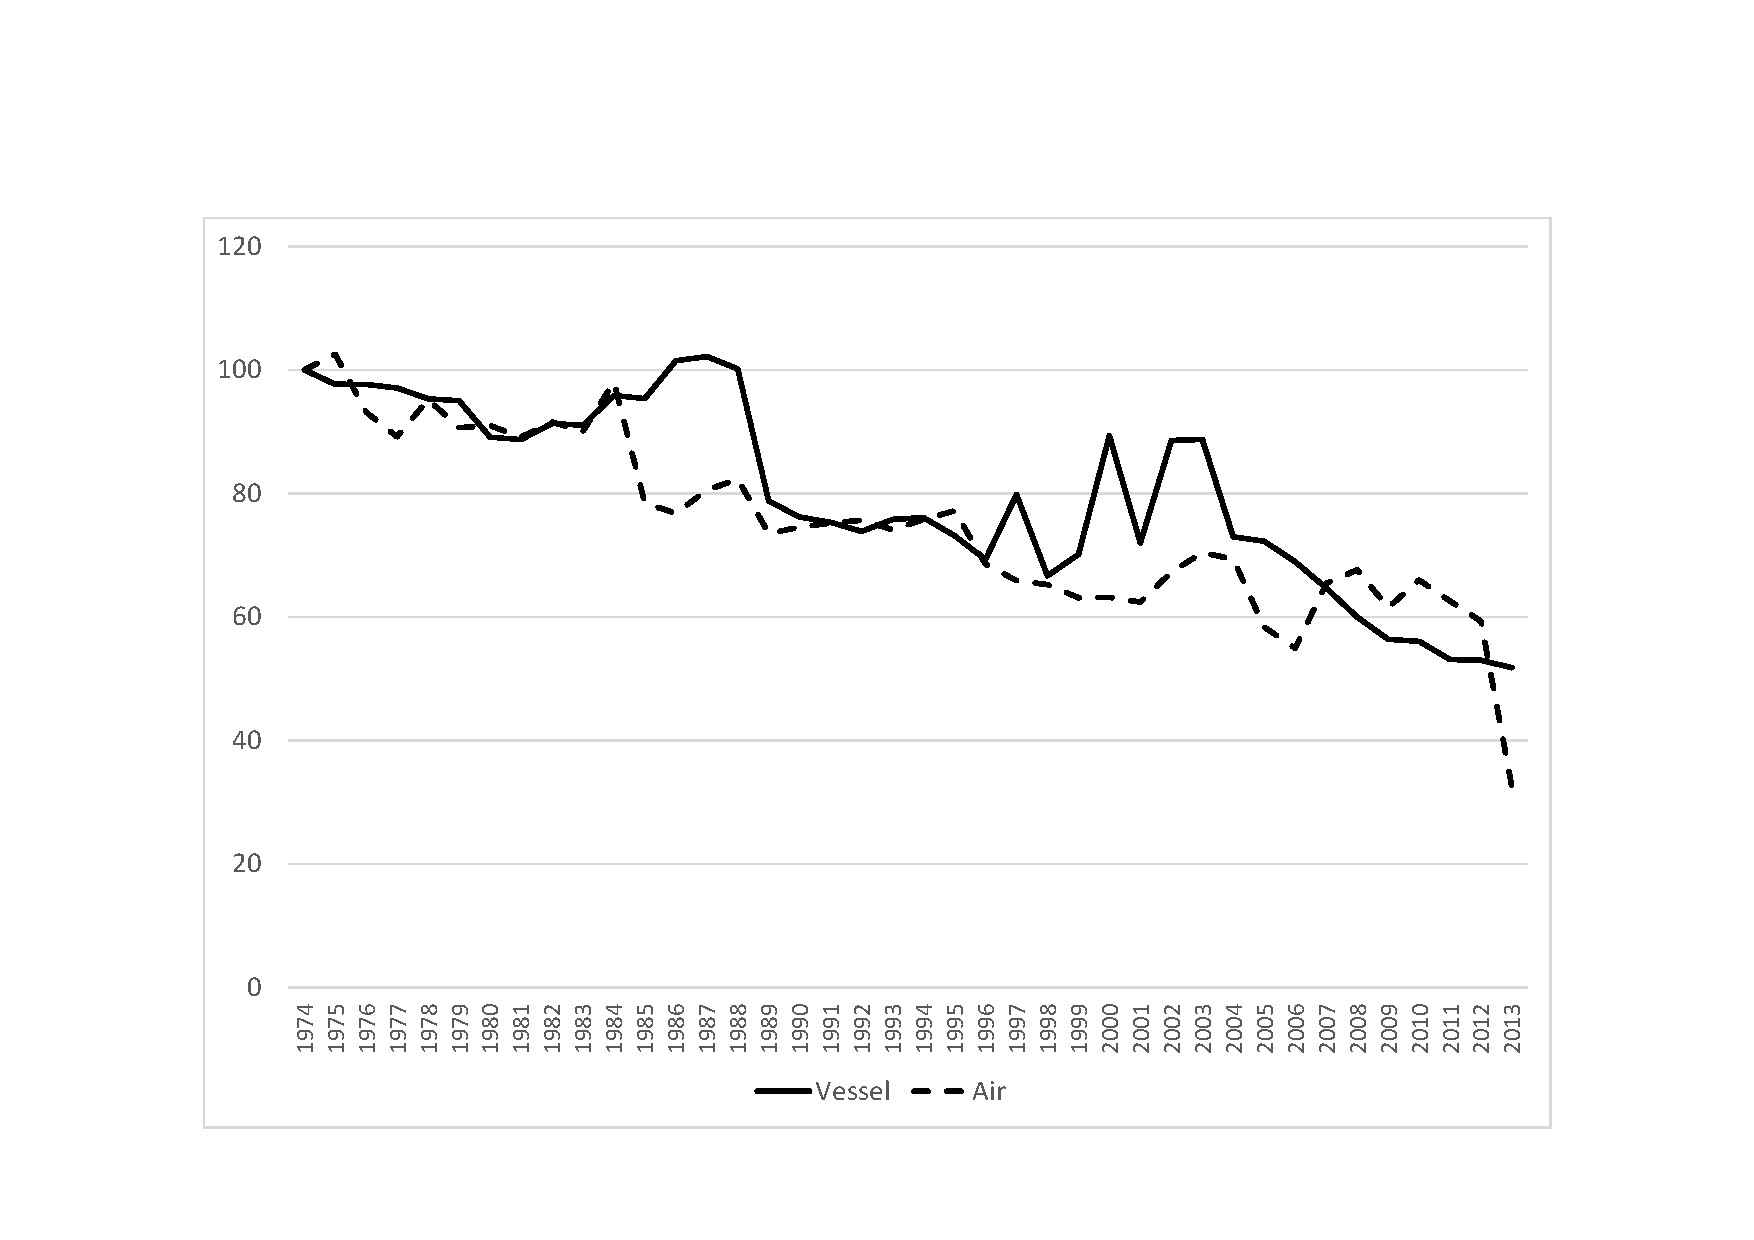
\includegraphics[width=5cm,height=5cm]{TC_addplusmult_compeffects_excl.pdf} \\
\end{tabular}
\end{center}
\end{figure}

\end{frame}

\begin{frame}[label=slide_comment_compositioneffects]
\frametitle{Two main findings}
\begin{itemize}
\item The importance of excluding composition effects  \vspace{0.1cm}
\begin{itemize}
\item[-] The reduction of the \textit{pure} transport costs: Starts in 1985 (not in 1974) \vspace{0.1cm}
\item[-] The reduction between 1974 and 1984 (\hyperlink{slide_fig1}{\beamergotobutton{Figure 1}}) is attributable to change in the composition of trade patterns \vspace{0.1cm}
\item[-] Overall (pure) transport costs have declined by $\simeq$ 40\% since 1985\vspace{0.1cm}
\end{itemize}
\item The importance of the additive component of transport costs (again) \vspace{0.1cm}
\begin{itemize}
\item[-] When only iceberg costs are modeled (Panel (a)): A stronger decrease in Air transport over the 1985-2005 period \vspace{0.1cm}
\item[-] In accordance with Hummels (2007), Behar \& Venables (2011) \vspace{0.1cm}
\item[-] But... No substantial difference when additive costs are included (Panel (b))
\end{itemize}
\end{itemize}
\end{frame}


\begin{frame}
\frametitle{Decomposing (\textit{pure}) transport costs over time }
\begin{figure}[htbp]
%\caption{Decomposing transport costs over time,
%composition effects excluded}
%\label{fig:TC_add_mult_compeffects_excl}
\begin{center}
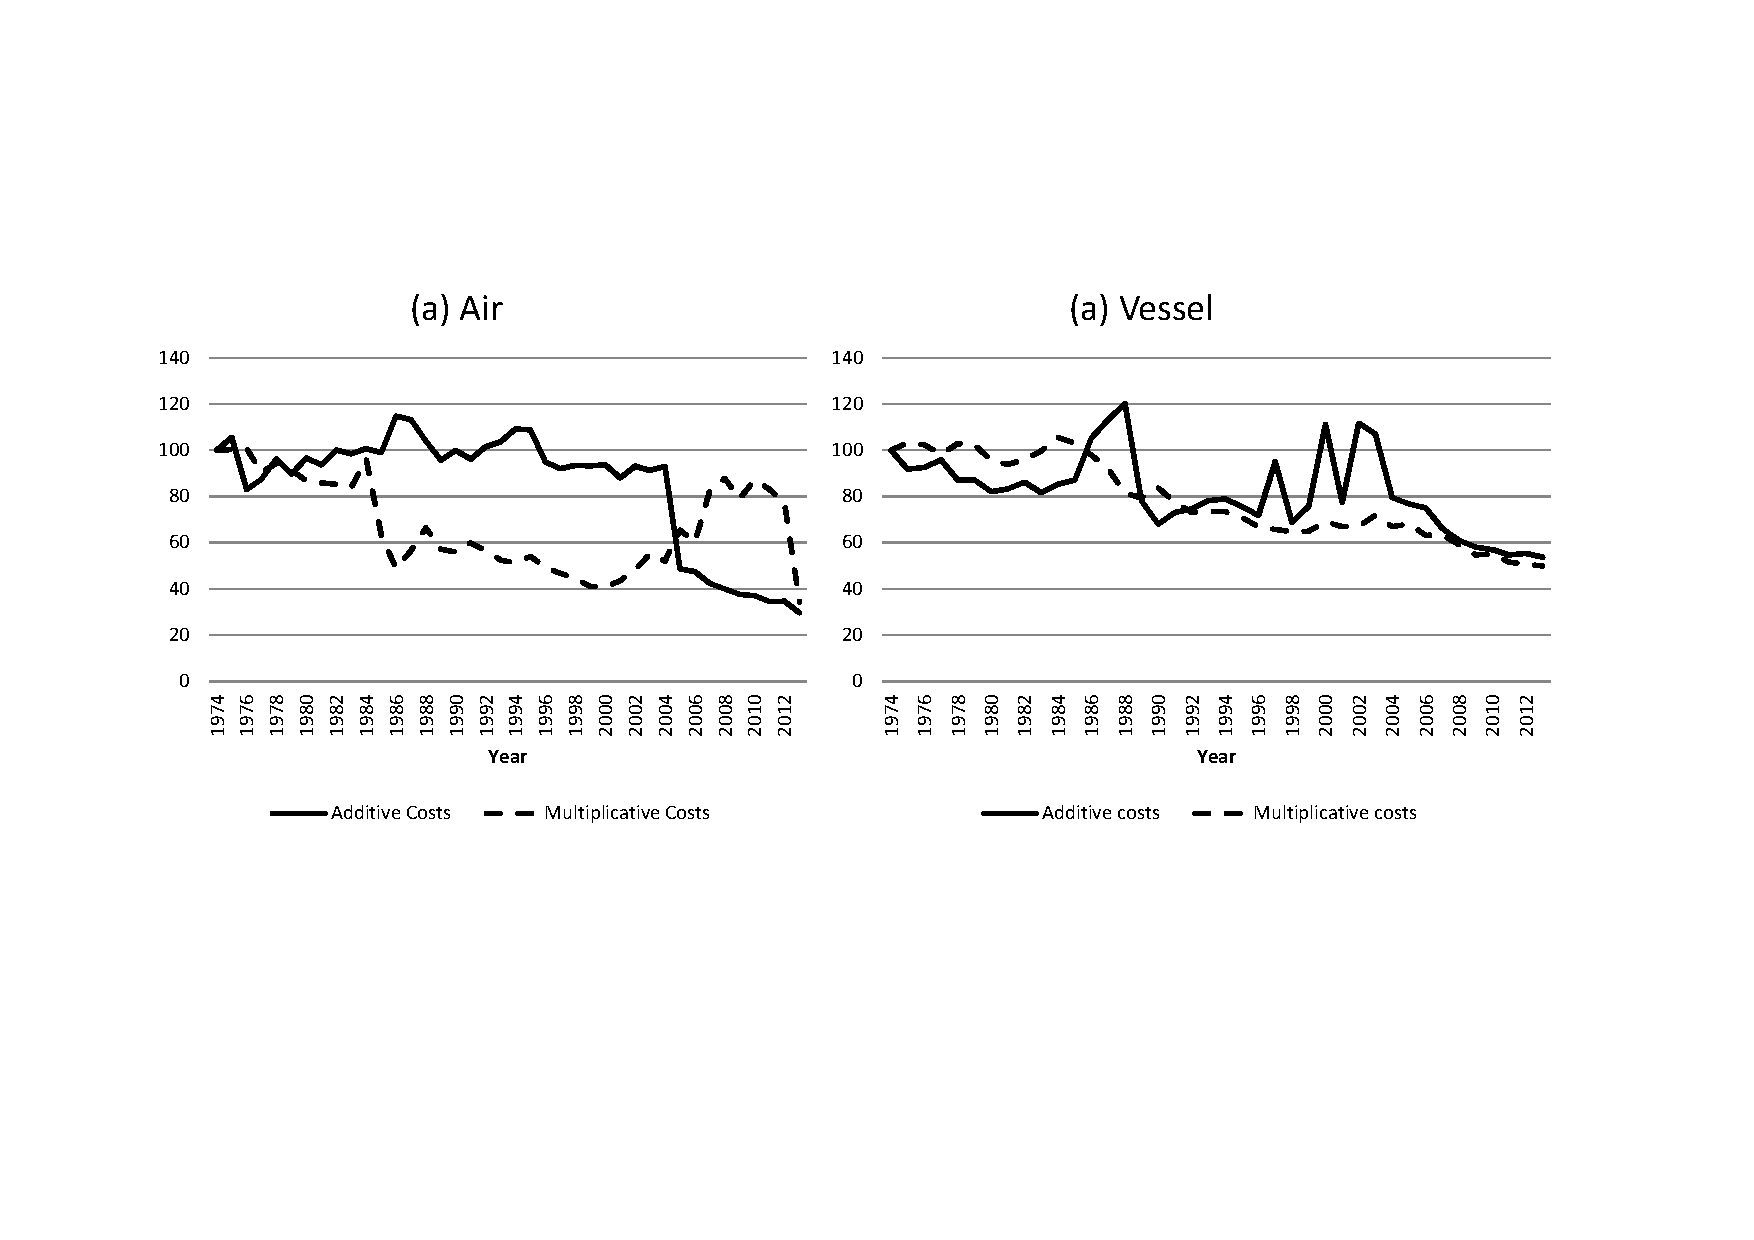
\includegraphics[width=8cm, height=3.5cm]{Fig3b_TCovertime_add_et_mult_3d.pdf}
%{\footnotesize {OECD data} }
\end{center}
\end{figure}
\begin{itemize}
\item For Vessel: Similar downward trend for both $\tau$ and $t$  \vspace{0.1cm}
\item For Air: Much more contrasted trends  \vspace{0.1cm}
\begin{itemize}
\item[-] Substantial decrease in the ad-valorem costs over 1985-2005, but roughly constant additive costs  \vspace{0.1cm}
\item[$\Rightarrow$] An explanation to the difference between Panels (a) and (b) above  \vspace{0.1cm}

\item[$\Rightarrow$] The importance of modeling additive costs  \vspace{0.1cm}
\item[-] Trend reversal around 2005: Any suggestion?
\end{itemize}
\end{itemize}
\end{frame}


\begin{frame}
\frametitle{Conclusion}
\textbf{Our paper: Empirical evidence about the role of the additive component in international transport costs} \vspace{0.1cm}
\begin{itemize}
\item Provide a quantitative evaluation of both the additive and the ad-valorem components \vspace{0.1cm}
\begin{itemize}
\item[-] Based on the US imports flows from 1974 to 2013 \vspace{0.1cm}
\item[-] Additive cost: amount to 2.8\% of the export price in ocean shipping, 1.8\% in air transport \vspace{0.1cm}
\item[-] Iceberg cost: 3.2\% and 2.5\% for air and ocean respectively \vspace{0.1cm}
\end{itemize}
\item The importance of taking into account additive transport costs \vspace{0.1cm}
\begin{itemize}
\item[-] Additive costs are far from negligible quantitatively \vspace{0.1cm}
\item[-] A better fit of the model when they are taken into account    \vspace{0.1cm}
\end{itemize}
\item Characterize the evolution of transport costs over time \vspace{0.1cm}
\begin{itemize}
\item[-] Importance of the composition effects \vspace{0.1cm}
\item[-] Biased picture of the time trends of transport costs in air when omitting the additive dimension
\end{itemize}
\end{itemize}

\end{frame}

\begin{frame}
\frametitle{Conclusion}

\textbf{Three main possible extensions}
\begin{itemize}
\item On the empirical side: \vspace{0.1cm}
\begin{itemize}
\item[(1)] Compare the trends in transports costs \textit{between} air and vessel (excluding composition effects) \vspace{0.1cm}
\item[(2)] Go deeper in the structural determinants of transport costs \vspace{0.1cm}
\begin{itemize} 
\item[$\star$] Identify the respective roles of handling costs, insurance and freight costs at the root of the import-export prices gap \vspace{0.1cm}
\end{itemize}
\end{itemize}
\item On the theoretical side: 
\begin{itemize}
\item[(3)]Use our results to explore the role of additive costs \vspace{0.1cm}
\begin{itemize}
\item[$\star$] In shaping international trade flows (trade theory) \vspace{0.1cm}
\item[$\star$] In affecting the international transmission of business cycles (business cycle theory)
\end{itemize}
\end{itemize}
\end{itemize}
\end{frame}

\beginbackup



\appendix
\begin{frame}[label=app_data]
\frametitle{More on our database}
\begin{itemize}
\item Implications (and limitations) \vspace{0.1cm}
\begin{itemize}
\item[-] Only cover international transport costs \vspace{0.1cm}
\item[-] Among transport costs, only quantitative costs (freight, insurance and handling - nothing about those related to the time value of goods) \vspace{0.1cm}
\end{itemize}
\item A rich database to exploit \vspace{0.1cm}
\begin{itemize}
\item[-] US imports, large time period: Broad view of international trade flows \vspace{0.1cm}
\item[-] A reliable database, already used by Hummels (2007). But we have a longer period of time \vspace{0.1cm}
\item[-] Have both the import and the export prices: Estimate both the levels of the ad-valorem and the additive trade costs ($\neq$ Irrarazabal et al., 2015)
\end{itemize}
\end{itemize}
\hyperlink{slide_data}{\beamergotobutton{Back to slide}}
\end{frame}

\begin{frame}[label=app_method_1]
\frametitle{More on the estimation strategy (1)}
\begin{itemize}
\item Assumptions on the specification of transport costs (as in Irrarazabal et al., 2015) \vspace{0.1cm}
\begin{itemize}
\item[-] Both iceberg and additive costs are separable between the origin country $i$ and the product $k$ dimensions \vspace{0.1cm}
\item[-] Separability in a multiplicative manner for ad-valorem costs and additive manner for per-kg costs \vspace{0.1cm}
\item[$\Leftrightarrow$] Write $t_{ik}$ and $\tau_{ik}$ as:
\begin{equation}
 \tau_{ik} = \tau_{i} \times \tau_{k}, \qquad t_{ik} = t_{i} + t_{k} \label{eq:specifTC}
 \end{equation}
\end{itemize}
\item Given the constraint $\frac{p_{ik}}{\widetilde{p}_{ik}} -1$, the error term should be always positive and multiplicative \vspace{0.1cm}
\item[$\Rightarrow$] The estimated equation becomes:
$$\frac{p_{ik}}{\widetilde{p}_{ik}}-1 =\left(\tau_{i} \times \tau_{k} -1+\frac{t_{i} + t_{k}}{\widetilde{p}_{ik}} \right)\times \exp(\epsilon_{ik})$$
\begin{itemize}
\item[-] With $\epsilon_{ik}$ following a normal law centered on 0.
\end{itemize}
\end{itemize}
\hyperlink{slide_method}{\beamergotobutton{Back to slide}}
\end{frame}



\begin{frame}[label=app_method_2]
\frametitle{More on the estimation strategy (2)}
\begin{itemize}
\item The non-linear least squares method \vspace{0.1cm}
\begin{itemize}
\item[-] At the basis of the method: Approximate the model by a linear one and refine the parameters by successive iterations \vspace{0.1cm}
\item[-] The criterion for convergence: That the sum of the squares of the residuals does not not increase? from one iteration to the next \vspace{0.1cm}
\end{itemize}
\item Eliminate potential influence of outliers: Exclude the 5 percent of the upper and lower tails of the distribution \vspace{0.1cm}
\item Obtaining the final estimates: More details  \vspace{0.1cm}
\begin{itemize}
\item[-] After estimating Equations (\ref{eq:model_with_add}) and (\ref{eq:model_nlI}), re-built \vspace{0.1cm}
\begin{itemize}
\item[$\star$] With additive costs:
$$\widehat{\tau}^{adv}_{ik} = \widehat{\tau_{i}} \times \widehat{\tau_{k}}, \qquad \widehat{t}^{add}_{ik} = \widehat{t}_{i} + \widehat{t}_{k}$$
\item[$\star$] With only iceberg costs:
$$\widehat{\tau}^{ice}_{ik} = \widehat{\tau_{i}} \times \widehat{\tau_{k}}$$
\end{itemize}
\item[-] Then, take the weighted average by country-product, \vspace{0.1cm}
\item[-] Using the values of each trade flow ($ik$-specific) over total yearly trade as a weighting scheme
\end{itemize}
\end{itemize}
\hyperlink{slide_method}{\beamergotobutton{Back to slide}}
\end{frame}

\begin{frame}[label=app_results_summary]
\frametitle{Decomposing transport costs: Summary \hyperlink{slide_results_summary}{\beamergotobutton{Back to slide}}}
\begin{table}[htbp]
  \centering
  \scriptsize{
  %\caption{Transport costs estimates: Summary \label{tab:summary_results}}
  \begin{center}
    \begin{tabular}{l|cc|cc}
      \hline \hline
    \multicolumn{5}{c}{Mean value over 1974-2013}   \\
    \# digit & \multicolumn{2}{c}{3 digits} & \multicolumn{2}{c}{4 digits ($^\ast$)} \\ \hline
    Mode  & Vessel & Air ($^{\ast \ast}$) & Vessel & Air \\ \hline
    \multicolumn{5}{l}{With only Ad-Valorem Trade Costs }  \\ \hline
    Mean  & 1.058 & 1.051 & 1.060 & 1.049 \\
    Median & 1.051 & 1.042 & 1.052 & 1.037 \\
    Std   & 0.032 & 0.042 & 0.036 & 0.045 \\
    Min. value & 1.003 & 1.001 & 1.003 & 1.000 \\
    Max. value & 1.304 & 1.685 & 1.408 & 2.051 \\ \hline
    \multicolumn{5}{l}{With Additive \& Ad-Valorem Trade Costs } \\ \hline
   \textit{Ad-valorem term} & & & & \\ \hline
    Mean  & 1.032 & 1.025 & 1.033 & 1.024 \\
    Median & 1.028 & 1.018 & 1.028 & 1.016 \\
    Std   & 0.023 & 0.023 & 0.025 & 0.026 \\
    Min. value & 1.001 & 1.000 & 1.000 & 1.000 \\
    Max. value & 1.227 & 1.474 & 1.264 & 1.537 \\ \hline
    \textit{Additive term }& & & &   \\ \hline
    Mean  & 0.029 & 0.018 & 0.028 & 0.019 \\
    Median & 0.019 & 0.007 & 0.017 & 0.008 \\
    Std   & 0.041 & 0.034 & 0.039 & 0.034 \\
    Min. value & 0.000 & 0.000 & 0.000 & 0.000 \\
    Max. value & 2.941 & 13.303 & 3.197 & 11.440 \\ \hline
        \# obs. & 29279 & 28207 & 29317 & 27680 \\
    \# origin country & 188 & 191 & 188 & 189 \\
    \# products & 230 & 211 & 666 & 567 \\  \hline \hline
  \end{tabular}
    \end{center}}
\parbox[l]{8cm}{\tiny{Notes: Statistics are obtained weighting each observation by its value. The additive term is expressed in fraction of fab price. ($^\ast$): Four 4-digit estimation: 0n selected years. ($^{\ast \ast}$): 1989 omitted in 3 digit estimation for air.}}
\end{table}%
\end{frame}





\begin{frame}[label=app_goodnessfit]
\frametitle{The role of additive costs: Goodness-of-fit evaluations}
\begin{itemize}
\item Provide a systematic diagnosis about the importance of additive costs  \vspace{0.1cm}
\item By comparing the goodness-of-fit of the regressions
\begin{itemize}
\item[-] Obtained under Specification (\ref{eq:model_nlI}) (no additive costs)
\item[-] vs Specification (\ref{eq:model_with_add}) (with additive costs) \vspace{0.1cm}
\end{itemize}
\item Various measures of goodness of fit
\begin{itemize}
\item[-] The $R^2$ (the larger the value, the better the fit) \vspace{0.1cm}
\item[-] Standard Error of Regression (SER) (the smaller the value, the better the fit) \vspace{0.1cm}
\item[-] The log-likelihood function and two derived measures, which take into account the degrees of freedom \vspace{0.1cm}
\begin{itemize}
\item[$\ast$] The Akaike Information Criterion (the lower AIC, the better the fit) \vspace{0.1cm}
\item[$\ast$] The log-likelihood ratio test ($H_0$: both models are equivalent)
\end{itemize}
\end{itemize}

\end{itemize}

\end{frame}

\begin{frame}
\frametitle{Goodness of fit comparison}
\begin{itemize}
\item Air, 3 digit - level, selected years
\end{itemize}
\begin{table}[htbp]
  \centering
 % \caption{Air: Measures of Goodness-of-fit (3 digits)}
  \scriptsize{
\begin{center}
    \begin{tabular}{l|ccccc|c}
    \hline \hline
    Year  &1980  & 1990  & 2000  & 2010 & 2013 & Mean stat \\ \hline
    \multicolumn{7}{l}{\bf{$R^2$} }\\ \hline
    Term I only &  0.27  & 0.25  & 0.32  & 0.42 & 0.34 & 0.31 \\
    Terms A \& I &  0.65  & 0.63  & 0.64  & 0.51 & 0.46 & 0.60 \\ \hline
    \multicolumn{7}{l}{\textbf{SER}  }  \\ \hline
    Term I only &  0.86  & 0.81  & 0.84  & 0.86 & 0.92 & 0.85 \\
    Terms A \& I &  0.71  & 0.67  & 0.70  & 0.79 & 0.85 & 0.73 \\ \hline
   \multicolumn{7}{l}{\textbf{AIC criteria}}  \\ \hline
    Term I only &  41171.0 & 60715.6 & 87492.6 & 102297.6 & 88191.9 & 70498.1 \\
    Terms A \& I & 35738.4 & 52098.9 & 74954.9 & 95887.1 & 80873.7 & 62285.0 \\ \hline
    \multicolumn{7}{l}{\textbf{Log-likelihood}} \\ \hline
    Term I only &  -20253.5 & -29977.8 & -43341.3 & -50746.8 & -43692.9 & -34888.6 \\
    Terms A \& I &  -17263.2 & -25393.5 & -36788.4 & -47277.5 & -39751.9 & -30508.3 \\
    LL ratio &  5980.6 & 9168.7 & 13105.7 & 6938.6 & 7882.1 & 8760.69 \\
    nb of restrictions & 369   & 393   & 426   & 426 & 427 & 402 \\
    p-value & 0.00 & 0.00 & 0.00 & 0.00 & 0.00 & 0.00 \\
    \hline \hline
 \end{tabular}%
    \end{center}}
  \label{tab:good_fit_air}%
 \parbox[l]{10cm}{\tiny{Notes: SER = Standard Error of regression; AIC = Akaike Information Criterion. $R^{2}$ between the log of predicted ratio and the log of the observed ratio. For the LL ratio test, the number of restrictions is equal to the number of parameters estimated, i.e., the number of partner countries plus the number of products. The mean statistics is calculated as the average value over all years. }}
\end{table}%
\hyperlink{slide_result2}{\beamergotobutton{Back to slide}}
\end{frame}

\begin{frame}
\frametitle{Goodness of fit comparison (cont')}
\begin{itemize}
\item Vessel, 3 digit - level, selected years
\end{itemize}
\begin{table}[htbp]
  \centering
  %\caption{Vessel: Measures of Goodness-of-fit (3 digits)}
    \scriptsize{
\begin{center}
\begin{tabular}{l|ccccc|c}
\hline \hline
Year  &  1980 & 1990 & 2000 & 2010  & 2013 & Mean stat \\ \hline
\multicolumn{7}{l}{\bf{$R^2$} }\\ \hline
Term I only &  0.415 & 0.456 & 0.401 & 0.350 & 0.339 & 0.39 \\
Terms A \& I &  0.575 & 0.590 & 0.571 & 0.491 & 0.462 & 0.56 \\ \hline
\multicolumn{7}{l}{\textbf{SER}  }  \\ \hline
    Term I only &  0.62 & 0.59 & 0.65 & 0.74  & 0.76 & 0.66 \\
    Terms A \& I &  0.53 & 0.51 & 0.55 & 0.66  & 0.68 & 0.57 \\ \hline
   \multicolumn{7}{l}{\textbf{AIC criteria}}  \\ \hline
    Term I only & 33010.3 & 51142.6 & 71365.9 & 84789.9 & 88191.9 & 57848.6 \\
    Terms A \& I &  28067.3 & 43664.7 & 60475.9 & 76161.3 & 80873.7 & 49682.3 \\ \hline
    \multicolumn{7}{l}{\textbf{Log-likelihood}} \\ \hline
    Term I only &  -16129.1 & -25169.3 & -35263.9 & -41998.9 & -43692.9 & -28534.3 \\
    Terms A \& I &  -13353.7 & -21171.4 & -29491.0 & -37418.7 & -39751.9 & -24151.3 \\
    LL ratio & 5550.96 & 7995.88 & 11545.98 & 9160.56 & 7882.15 & 8766.0 \\
    nb of restrictions  &  395 & 411 & 436 & 424   & 427 & 417 \\
    p-value & 0.00 & 0.00 & 0.00 & 0.00  & 0.00 & 0.00 \\
    \hline \hline
    \end{tabular}%
    \end{center}}
  \label{tab:good_fit_vessel}%
  \parbox[l]{10cm}{\tiny{Notes: SER = Standard Error of regression; AIC = Akaike Information Criterion. $R^{2}$ between the log of predicted ratio and the log of the observed ratio. For the LL ratio test, the number of restrictions is equal to the number of parameters estimated, i.e., the number of partner countries plus the number of products. The mean statistics calculated as the average value over all years. }}
\end{table}%
\hyperlink{slide_result2}{\beamergotobutton{Back to slide}}
\end{frame}


\begin{frame}[label=app_fig1]
\frametitle{Ad-valorem costs over time \hyperlink{slide_fig1}{\beamergotobutton{Back to slide}}}
\begin{figure}[htbp]
\caption{Ad-valorem Costs (Yearly mean value, 3 digits)}
\label{fig:mult_alone_withadd}
\begin{center}
\begin{tabular}{cc}
{\small (a) Air } & {\small (b) Vessel}\\
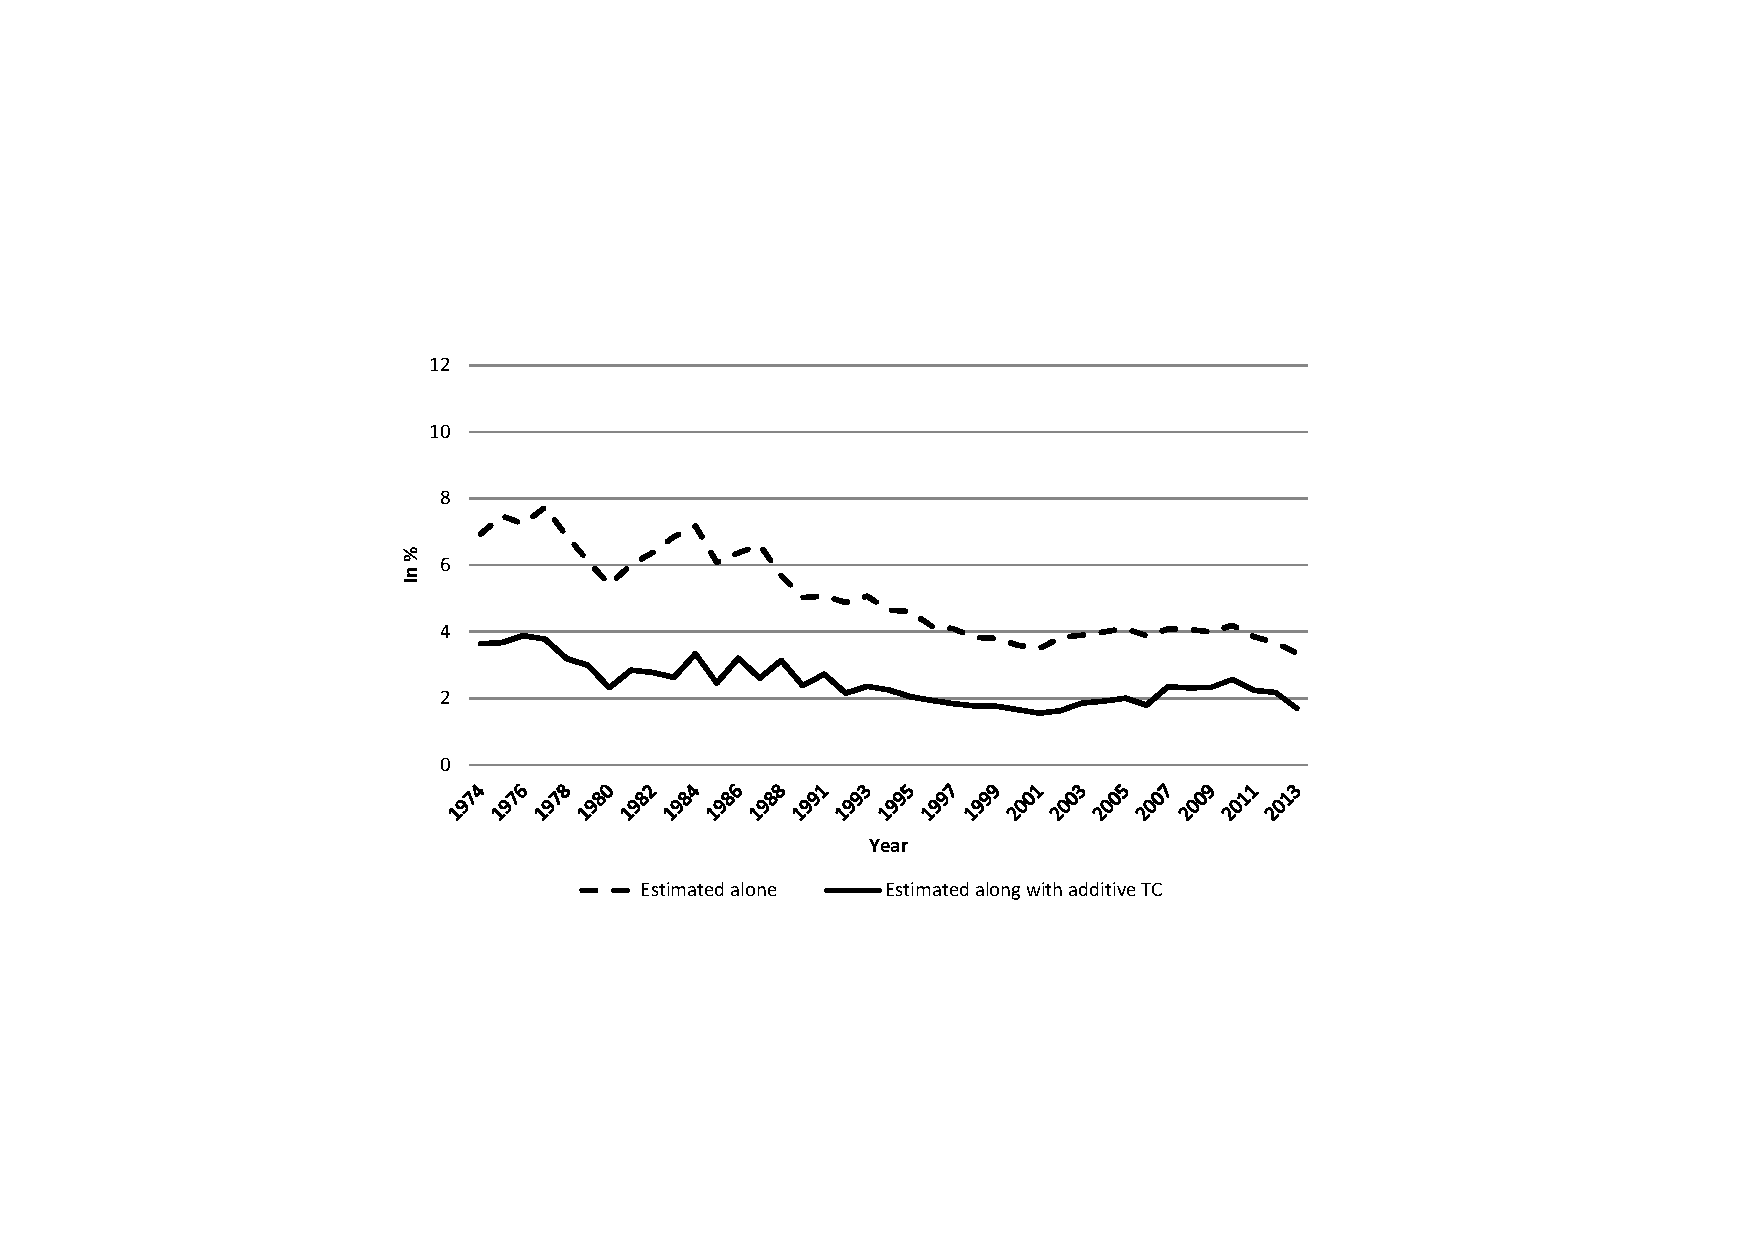
\includegraphics[width=5cm, height=2.5in]{Fig1a_mult_air_3d.pdf}
& 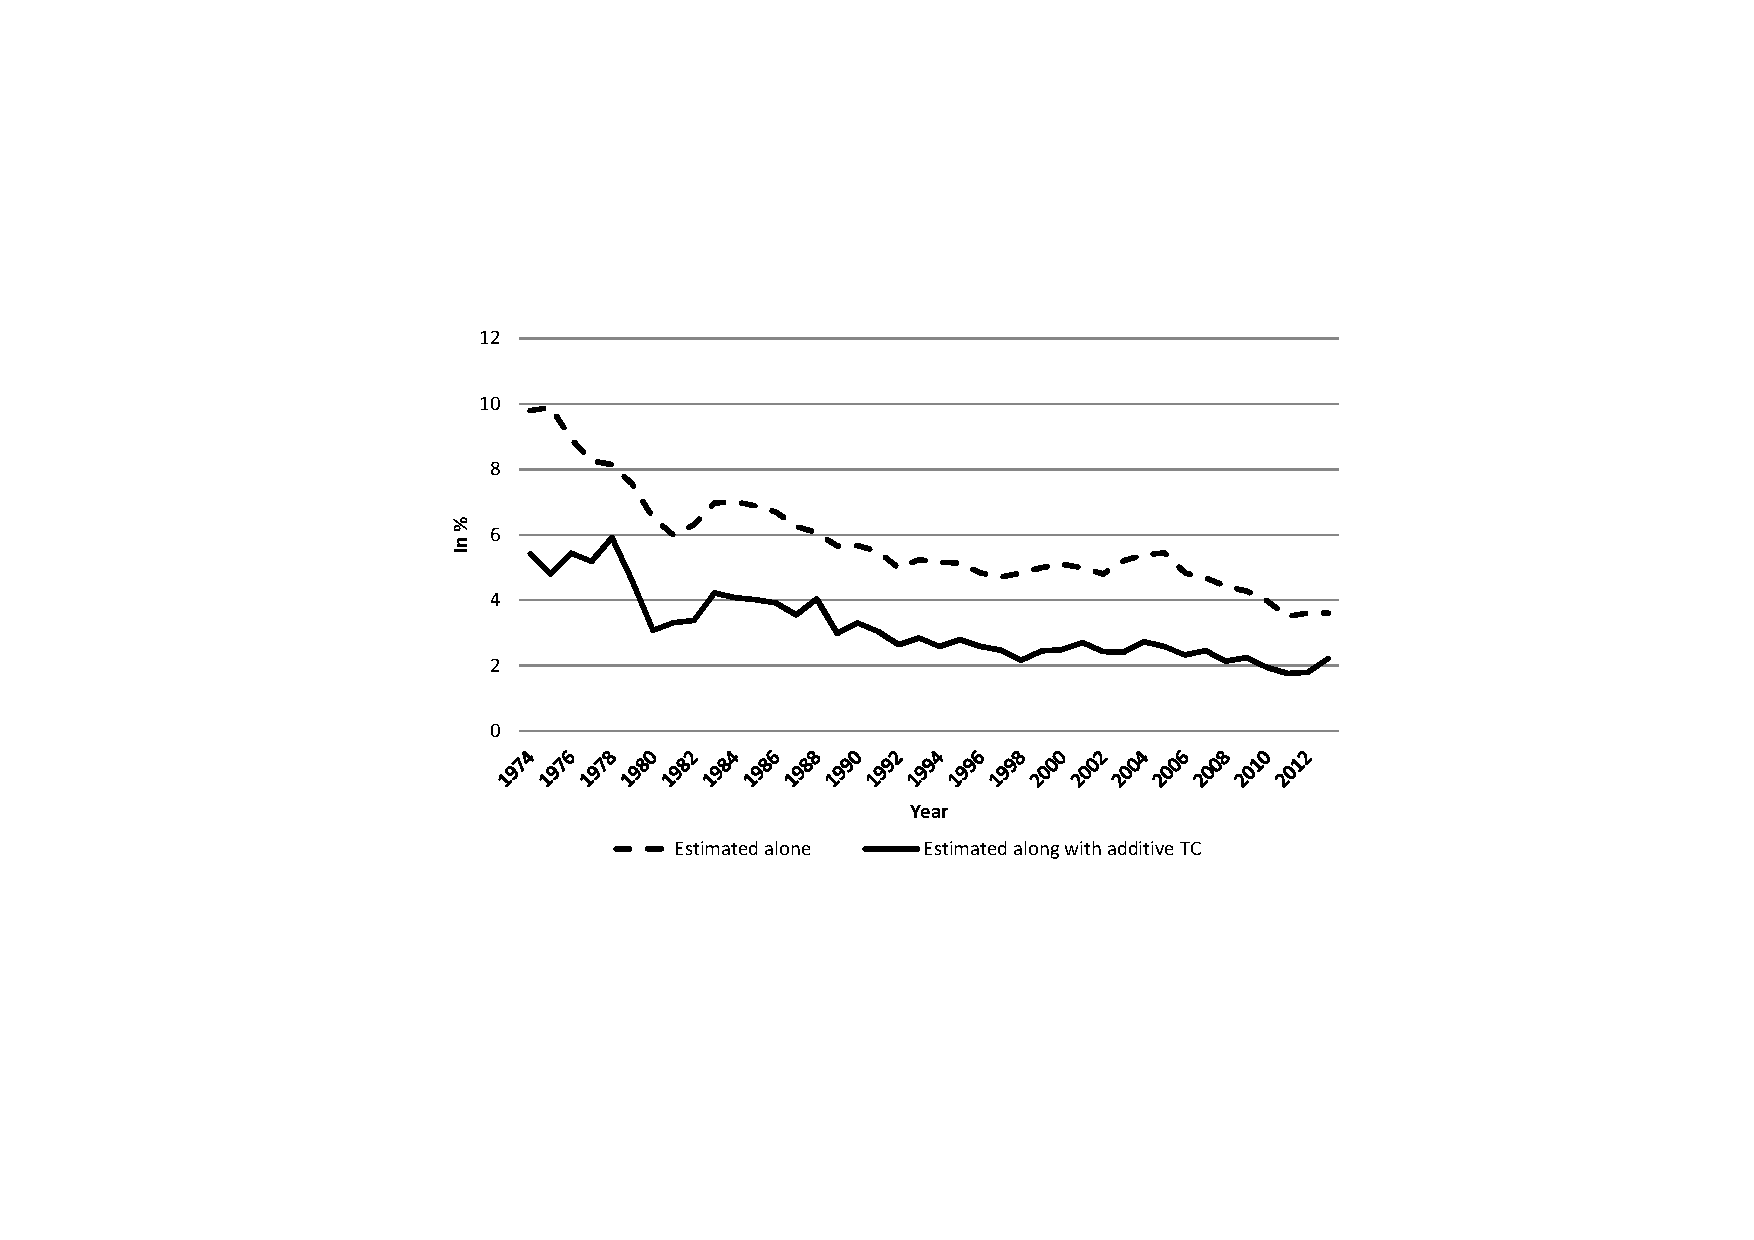
\includegraphics[width=5cm,height=2.5in]{Fig1b_mult_vessel_3d.pdf} \\
\end{tabular}
\end{center}
\end{figure}

\end{frame}

\begin{frame}[label=app_compositioneffects]
\frametitle{Excluding the composition effects of transport costs changes}
\begin{itemize}
\item For the ad-valorem component, we estimate the following equation:
\scriptsize
\begin{eqnarray}
\widehat{\tau}_{ikt}&=&\delta\times \exp\left(\sum_{i \neq \text{AFG}}\alpha_i.\mathbb{1}_i\right).\exp\left(\sum_{k\neq \text{011}}\beta_k.\mathbb{1}_k\right).\exp\left(\sum_{t \neq 1974}\gamma_t.\mathbb{1}_t\right) .\exp\left(\epsilon_{ikt}\right) \notag \\
\Leftrightarrow \ln(\tau_{ikt})&=&\delta +\sum_{i \neq \text{AFG}}\alpha_i.\mathbb{1}_i + \sum_{k\neq \text{011}}\beta_k.\mathbb{1}_k + \sum_{t \neq 1974}\gamma_t.\mathbb{1}_t+\epsilon_{ikt} \label{eq:compeffects_mult}
\end{eqnarray}
\normalsize
\begin{itemize}
\item[-] With $\widehat{\tau}_{ikt} = \widehat{\tau}^{ice}_{ikt}, \widehat{\tau}^{adv}_{ikt}$ previously obtained  \vspace{0.1cm}
\end{itemize}
\item For the additive component:
\scriptsize
\begin{eqnarray}
\widehat{t}_{ikt}&=&\left( \prod_{i \neq \text{ARG}}  \alpha_i.\mathbb{1}_i+\prod_{k}\beta_k.\mathbb{1}_k\right).\exp\left(\sum_{t \neq 1974}\gamma_t.\mathbb{1}_t\right) .\exp\left(\epsilon_{ikt}\right) \notag \\
\Leftrightarrow \ln(t_{ijt})&=&\ln\left( \prod_{i \neq \text{ARG}}  \alpha_i.\mathbb{1}_i+\prod_{k}\beta_k.\mathbb{1}_k\right) + \sum_{t \neq 1974}\gamma_t.\mathbb{1}_t+\epsilon_{ijt} \label{eq:compeffects_add}
\end{eqnarray}
\normalsize
\end{itemize}

\end{frame}

\begin{frame}
\begin{itemize}
\item More on the estimation method
\begin{itemize}
\item[-] Equations (\ref{eq:compeffects_mult}) and (\ref{eq:compeffects_add}): Preserve our specification of the ad-valorem and the additive costs (Equation (\ref{eq:specifTC})) \vspace{0.1cm}
\item[-] Equation (\ref{eq:compeffects_mult}) estimated using OLS, \vspace{0.1cm}
\item[-] Equation (\ref{eq:compeffects_add}) using non-linear least squares (by transport mode) \vspace{0.1cm}
\end{itemize}
\item Exclude the composition effects of transport costs changes $\Leftrightarrow$ Isolate the change in the time dimension  \vspace{0.1cm}
\begin{itemize}
\item[-] From the ad-valorem component estimation (Equation (\ref{eq:compeffects_mult})), build the variable $\Gamma_t$ ($\forall~t \geq 1974$):
\begin{equation*}
\Gamma_t = 100.\frac {\bar{\tau}_{1974}.\exp(\gamma_t)-1} {\bar{\tau}_{1974}-1}
\end{equation*}
\item[-] For the additive cost, we build the variable ($\forall~t \geq 1974$)
$$\Gamma^{add}_t = 100 \exp(\gamma_t)$$
\end{itemize}
\item The $\Gamma^{add}_t$ and $\Gamma_t$ series: Interpretation in percentage changes
\begin{itemize}
\item[] with an initial value of 100 for $t=1974$
\end{itemize}


\end{itemize}
 \hyperlink{slide_compositioneffects}{\beamergotobutton{Back to slide}}
\end{frame}


\end{document}
